% !TeX spellcheck = cs_CZ
%{\tikzset{external/prefix={tikz/FYZII/}}
% \tikzset{external/figure name/.add={ch17_}{}}
%---------------------------------------------------------------------------------------------------
% file fey2ch17.tex
%---------------------------------------------------------------------------------------------------
%====================Kapitola: Zákony elektromagnetické indukce ====================================
\setchaptertoc
\chapter{Zákony elektromagnetické indukce}\label{fyz:IIchapXVII}


\section{Fyzika elektromagnetické indukce}\label{fyz:IIchapXVIIsecI}
  V předcházející části jsme popsali mnoho jevů, které poukazovaly na to, jak složité a zajímavé 
  jsou jevy elektromagnetické indukce. Nyní bychom mohli pohovořit o základních principech, které 
  za těmito jevy stojí. Už jsme definovali emn ve vodivém obvodu jako celkovou sílu působící na 
  náboje, akumulovanou po celé délce obvodu. Přesněji je to tangenciální složka síly na jednotkový 
  náboj, integrovaná podél vodiče po celém obvodu. Tato veličina je proto rovna celkové práci 
  konané na jednotkovém náboji, jenž jednou prochází po obvodu.
  
  Uvedli jsme pravidlo toku, které říká, že emn je rovno rychlosti změny magnetického toku 
  takovýmto vodivým obvodem. Podívejme se na příčiny tohoto jevu. Nejdříve vezmeme v úvahu případ, 
  kdy se tok mění proto, že se část obvodu pohybuje v konstantním poli.

  \begin{figure}[ht!]  %\ref{fyz:fig332}
    \centering
    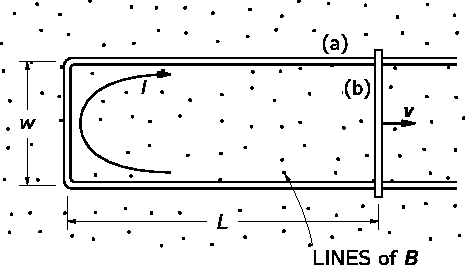
\includegraphics[width=0.8\linewidth]{fyz_fig332.pdf}
    \caption{Mění-li se v důsledku změny plochy obvodu magnetický tok, indukuje se ve smyčce emn. 
             (\cite[s.~294]{Feynman02}).}
    \label{fyz:fig332}
  \end{figure}
  
  Na obr. \ref{fyz:fig332} je znázorněna jednoduchá smyčka z drátu, jejíž rozměry jsou měnitelné. 
  Smyčka má dvě části, pevnou část (a) ve tvaru U a pohyblivou příčnou část (b), která může klouzat 
  podél dvou ramen U. Vždy je tam úplný obvod, ale jeho plocha se mění. Nyní umístíme smyčku do 
  homogenního magnetického pole tak, aby rovina U byla kolmá k poli. Podle pravidla se při pohybu 
  příčky objeví v smyčce emn, které je úměrné rychlosti změny toku smyčkou. Toto emn způsobí ve 
  smyčce proud. Budeme předpokládat, že vodič má dost velký odpor, a proto jsou proudy malé.
  
  Potom můžeme magnetické pole tohoto proudu zanedbat. Ve shodě s označením na obrázku bude tok 
  smyčkou roven \(wlB\), a proto pravidlo toku poskytuje následující vztah pro emn, které 
  budeme označovat symbolem \(\mathscr{E}\):  
  \begin{equation}\label{fyz:eq376}
    \mathscr{E} = wB\der{l}{t} = wBv
  \end{equation}
  
  (\(v\) je rychlost posunu příčky). Tento výsledek však musí být možné vysvětlit i tehdy, když 
  uvažujeme magnetickou sílu \(\vec{v}\times\vec{B}\) působící na náboje v pohybující se příčce. 
  Tyto náboje pocítí sílu, která je k vodiči tangenciální a která je rovna \(Bv\) případě 
  jednotkového náboje. Je konstantní podél příčky v délce \(w\) všude jinde je nulová, takže 
  integrál je roven
  \begin{equation}\label{fyz:eq377}
    \mathscr{E} = wvB,
  \end{equation}
  což je stejný výsledek, jako jsme dostali z rychlosti změny toku.
  
  Tuto argumentaci lze rozšířiti na každý takový případ, kdy máme konstantní magnetické pole a 
  vodiče se pohybují. Obecně je možné dokázat, že v každém obvodě, jehož části se pohybují v 
  konstantním magnetickém poli, je emn rovno časové derivaci magnetického toku bez ohledu na tvar 
  obvodu.
  
  Co se však stane tehdy, když smyčka stojí a mění se magnetické pole? Odpověď na tuto otázku není 
  možné získat stejným způsobem. Faraday však zjistil (z experimentu), že pravidlo toku platí bez 
  ohledu na to, co je příčinou změny toku. Síla působící na elektrické náboje je zcela obecně dána 
  výrazem \(\vec{F}=q(\vec{E}+ \vec{v}\times\vec{B})\); nevyskytují se tam žádné zvláštní „síly 
  pocházející od změn magnetických polí“. Každá síla působící na náboje v nepohyblivém vodiči 
  pochází od členu \(\vec{E}\). Faradayova pozorování vedla k poznatku, že elektrická a magnetická 
  pole jsou vázána novým zákonem: v oblasti, kde se s časem mění magnetické pole, vznikají 
  elektrická pole. Právě toto elektrické pole pohání elektronyvodičem, a je tak odpovědné za emm v 
  nehybném obvodu, měníli se tam magnetický tok.
  
  Obecný zákon pro elektrické pole související s měnícím se magnetickým polem má tvar
  \begin{equation}\label{fyz:eq378}
    \nabla\times\vec{E} = -\pder{\vec{B}}{t}
  \end{equation}
  a nazývá se \textbf{Faradayův zákon}. Objevil ho Faraday, ale v diferenciální formě jej poprvé 
  uvedl Maxwell jako jednu ze svých rovnic. Všimněme si, jak z tohoto zákona vyplývá pravidlo toku 
  pro obvody. 
  
  Použitím Stokesovy věty můžeme tento zákon přepsat do integrální formy
  \begin{equation}\label{fyz:eq379}
    \oint_\Gamma\vec{E}\cdot\dd{\vec{s}} 
      = -\pder{ }{t}\int_S\vec{B}\cdot\vec{n}\dd{S} = -\int_S\pder{B}{t}\cdot\vec{n}\dd{S}
  \end{equation}
  kde jako obvykle, je \(\Gamma\) libovolná uzavřená křivka a \(S\) libovolná plocha ohraničená 
  touto křivkou. Musíme mít na zřeteli, že je matematická křivka fixovaná v prostoru a S je pevná 
  plocha. Pak je možné dát časovou derivaci před integrál, čímž dostaneme
  \begin{equation}\label{fyz:eq380}
    \oint_\Gamma\vec{E}\cdot\dd{\vec{s}} 
      = -\int_S\pder{B}{t}\cdot\vec{n}\dd{S} = -\pder{ }{t}(\text{tok plochou S})
  \end{equation}
  Aplikujeme-li tento vztah na křivku \(\Gamma\), která prochází podél \emph{pevného} obvodu 
  vodičů, dostaneme opět „pravidlo toku“. Integrál na levé straně představuje emn a na pravé straně 
  je záporně vzatá změna toku procházejícího plochou, jíž ohraničuje křivka. Rovnice 
  (\ref{fyz:eq378}) aplikovaná na pevný obvod je rovnocenná s pravidlem toku. Pravidlo toku 
  (říkající, že emn v obvodu je rovno rychlosti změny magnetického toku obvodem) platí tedy bez 
  ohledu na to, zda se tok mění v důsledku změn pole nebo v důsledku pohybu obvodu (nebo 
  probíhají-li obě změny). Tyto dvě možnosti - pohyb obvodu nebo změny pole - nejsou v tvrzení 
  pravidla rozlišeny. V našem vysvětlení pravidla jsme však použili dva zcela rozdílné zákony pro 
  dva případy: \(\vec{v}\times\vec{B}\) pro pohyb obvodu a \(\nabla\times\vec{E} = -\pder{B}{t}\) 
  pro změny pole.
  
  Ve fyzice neznáme žádný jiný takový jednoduchý a přesný obecný princip, který by ke skutečnému 
  pochopení vyžadoval analýzu \emph{dvou rozdílných jevů}. Obvykle takové krásné zobecnění pochází 
  z jediného hlubokého, základního principu. Ale v tomto případě žádný takový hluboký důsledek 
  nějakého principu nemáme. Toto pravidlo musíme chápat jako kombinaci dvou zcela odlišných jevů.
  
  Pravidlo toku musíme chápat následujícím způsobem. Obecně je síla na jednotkový náboj rovna 
  \(\vec{F}/q = \vec{E}+\vec{v}\times\vec{B}\). V pohybujících se vodičích se objevuje síla 
  vyjádřená druhým členem. Kromě toho vzniká pole \(\vec{E}\) jestliže se někde se mění magnetické 
  pole. Tyto jevy jsou nezávislé, ale emn podél vodivé smyčky je vždy rovno rychlosti změny 
  magnetického toku smyčkou.
  
\section{Výjimky z pravidla toku}\label{fyz:IIchapXVIIsecII}
  Uveďme několik příkladů pocházející částečně od Faradaye, z nichž je vidět, jak je důležité 
  rozlišovat tyto dva jevy, odpovědné za indukované emm. Naše příklady zahrnují situace, v nichž 
  pravidlo toku neplatí buď proto, že nemáme žádný vodič, nebo proto, že dráha sledovaná 
  indukovanými proudy se v objemu vodiče přemisťuje.

  Začneme důležitou poznámkou: Ta část emm, která pochází od pole \(\vec{E}\), nezávisí na 
  existenci fyzického vodiče (na rozdíl od té části, která pochází od \(\vec{v}\times\vec{B}\)). 
  Pole \(\vec{E}\) může existovat i v prázdném prostoru a jeho křivkový integrál po libovolné 
  křivce, kterou si představíme pevně v prostoru, je roven rychlosti změny toku \(\vec{B}\) touto 
  křivkou. (Všimněme si, že je to úplně jinak než u pole \(\vec{E}\) vytvářeném statickými náboji, 
  když byl křivkový integrál \(\vec{E}\) po uzavřené smyčce vždy nulový.)

  \begin{figure}[ht!]  %\ref{fyz:fig333}
    \centering
    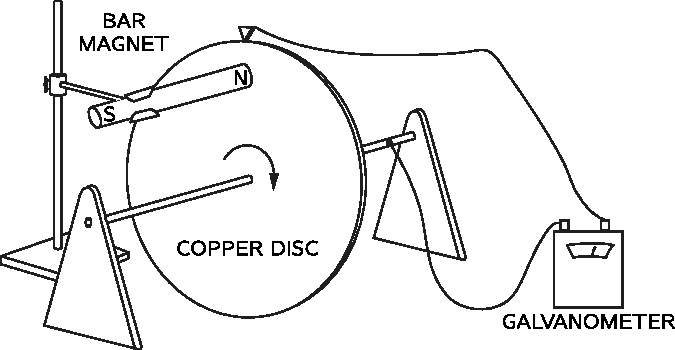
\includegraphics[width=0.9\linewidth]{fyz_fig333.pdf}
    \caption{Při otáčení kotouče vzniká emn pocházející od \(\vec{v}\times\vec{B}\), ale tok se 
             přitom nemění.
             (\cite[s.~296]{Feynman02}).}
    \label{fyz:fig333}
  \end{figure}
  
  Nyní popíšeme případ, kdy se tok obvodem nemění, a přece existuje emn. Na obr. \ref{fyz:fig333} 
  je znázorněn vodivý kotouč, který je umístěn v magnetickém poli a může se otáčet kolem pevné osy. 
  Jeden kontakt je přiložen k ose a druhý je opřen o vnější okraj kotouče. Obvod je uzavřen 
  galvanometrem. Když se kotouč otáčí, zůstává „obvod“ - ve smyslu místa v prostoru, kterým tečou 
  proudy - stále stejný. Část obvodu však prochází kotoučem, tedy materiálem, kterým se pohybuje. 
  Ačkoli je tok „obvodem“ konstantní, bude v obvodu emn, o čemž je možné se přesvědčit sledováním 
  výchylky galvanometru.Je jasné, že máme případ, kdy síla \(\vec{v}\times\vec{B}\) v pohybujícím 
  se kotouči vyvolává emm, které není možné přiřadit změně toku.
  
  \begin{figure}[ht!]  %\ref{fyz:fig334}
    \centering
    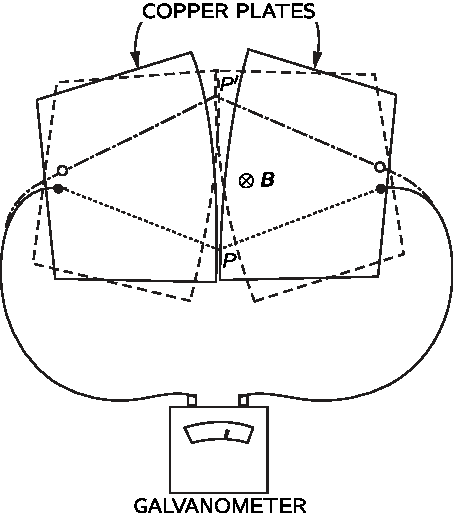
\includegraphics[width=0.8\linewidth]{fyz_fig334.pdf}
    \caption{Při pootočení destiček v homogenním magnetickém poli se tok může silně změnit, ale emn
             nevzniká
             (\cite[s.~296]{Feynman02}).}
    \label{fyz:fig334}
  \end{figure}
  
  Opačným příkladem je dost neobvyklá situace, kdy se tok „obvodem“ (opět ve smyslu místa, v němž 
  je proud) mění, ale nemáme tam emn. Představme si dvě kovové destičky s mírně zakřivenými okraji, 
  které znázorňuje obr. \ref{fyz:fig334} a které jsou umístěny v homogenním magnetickém poli kolmém 
  k jejich povrchu. Tak, jak je znázorněno na obrázku, je každá z destiček připojena ke 
  galvanometru. Destičky se v jednom bodě \(P\) dotýkají, čímž je vytvořen uzavřený obvod. 
  Otočíme-li destičky o malý úhel, posune se jejich styčný bod do bodu \(P\). Představíme-li 
  si „obvod“ tak, že se uzavírá destičkami tam, kde prochází na obrázku přerušovaná čára, mění se 
  při otáčení destiček velmi výrazně magnetický tok procházející tímto obvodem. Natáčení lze 
  provést velmi pomalými pohyby, při nichž je \(\vec{v}\times\vec{B}\) nepatrné a emn prakticky 
  neexistuje. Pravidlo toku však v tomto případě neplatí. Lze jej aplikovat pouze na obvody, v 
  nichž se nemění materiál obvodu. Při změně materiálu obvodu se musíme vrátit k základním zákonům. 
  Správný fyzikální obsah je vždy dán dvěma základními zákony
  
  \begin{align*}
    q(\vec{E} + \vec{v}\times\vec{B}) &=  \vec{F}   \\
                  \nabla\times\vec{E} &= -\pder{\vec{B}}{t}.
  \end{align*}

\section{Urychlování částic indukovaným polem. Betatron}\label{fyz:IIchapXVIIsecIII}
  Už jsme hovořili o tom, že elektromotorické napětí generované měnícím se magnetickým polem může 
  existovat i bez vodičů; můžeme mít elektromagnetickou indukci i bez drátů. Můžeme si představit 
  emn podél libovolné matematické křivky v prostoru. Je definováno jako tangenciální složka 
  \(\vec{E}\) integrovaná po křivce. Faradayův zákon říká, že tento křivkový integrál je roven 
  rychlosti změny magnetického toku uzavřenou křivkou (vztah \ref{fyz:eq380}).
  
  Jako příklad působení takového indukovaného elektrického pole budeme nyní uvažovat pohyb 
  elektronů v proměnném magnetickém poli. Představme si magnetické pole, jež má všude v rovině 
  vertikální směr (obr. \ref{fyz:fig335}). Magnetické pole je vytvořeno elektromagnetem, ale takové 
  podrobnosti nás nebudou zajímat. Budeme však předpokládat, že jde o magnetické pole, které je 
  vzhledem k nějaké ose symetrické, tj. že intenzita magnetického pole závisí pouze na vzdálenosti 
  od této osy.

  \begin{figure}[hb!]
    \centering
    \subcaptionbox{\label{fyz:fig335a}}{\luafigure[0.9]{fyz_fig335a.pdf}}              \\
    \subcaptionbox{\label{fyz:fig335b}}{\luafigure[0.9]{fyz_fig335b.pdf}}
    \caption{Elektron je urychlován v osově symetrické časově proměnném magnetickém poli
             (\cite[s.~297]{Feynman02}).}
    \label{fyz:fig335}
  \end{figure}
  
  Magnetické pole se mění i v čase. Dále si představíme elektron, který se pohybuje v tomto poli po 
  kruhové dráze s konstantním poloměrem. Střed dráhy leží na zmíněné ose. (Později uvidíme, jak 
  může být takový pohyb uskutečněn.) V důsledku měnícího se magnetického pole bude existovat 
  elektrické pole \(\vec{E}\) tangenciální k trajektorii elektronu, a to bude způsobovat pohyb 
  elektronu po kružnici. Má-li trajektorie elektronu poloměr \(r\), bude křivkový integrál 
  \(\vec{E}\) podél trajektorie rovem hodnotě \(E\) násobené obvodem kruhu \(2\pi r\). Magnetický 
  tok je obecně dán integrálem. Předpokládáme-li, že \(B_{\text{stř}}\) je střední magnetické pole 
  uvnitř kruhu, je tok roven součinu tohoto středního magnetického pole a plochy kruhu. Tak 
  dostaneme
  \begin{equation*}
    2\pi rE = \der{}{t}(B_\text{stř}\cdot\pi r^2)
  \end{equation*}
  
  Protože předpokládáme konstantní \(r\), bude \(E\) úměrné časové derivaci středního pole:
  \begin{equation}\label{fyz:eq381}
    E = \frac{r}{2}\der{B_{\text{stř}}}{t}.
  \end{equation}
  Elektron pocítí elektrickou sílu \(qE\) a bude urychlován. Uvědomíme-li si, že relativisticky 
  správná pohybová rovnice dává rychlost změny hybnosti úměrnou síle, dostaneme
  \begin{equation}\label{fyz:eq382}
    qE = \der{p}{t}.
  \end{equation}
  
  Pro kruhovou trajektorii jsme předpokládali, že elektrická síla působící na elektron má vždy směr 
  jeho pohybu, a proto bude celková hybnost růst rychlostí určenou rovnicí (17.5). Zkombinováním 
  vztahů (\ref{fyz:eq382}) a (\ref{fyz:eq381}) můžeme vyjádřit rychlost změny hybnosti pomocí změny 
  středního magnetického pole:
  \begin{equation}\label{fyz:eq383}
    \der{p}{t} = \frac{qr}{2}\cdot\der{B_{\text{stř}}}{t}.
  \end{equation}
   Integrujeme-li tento vztah podle \(t\), dostaneme pro hybnost elektronu vyjádření
  \begin{equation}\label{fyz:eq384}
    p = p_0 + \frac{qr}{2}\Delta B_{\text{stř}},
  \end{equation}
  kde \(p_0\) je počáteční hybnost elektronu a \(\Delta B_{\text{stř}}\) je změna 
  \(B_{\text{stř}}\). Na této myšlence je založena činnost \textbf{betatronu} - zařízení k 
  urychlování elektronů na velké energie.
   
  Abychom podrobně pochopili, jak betatron pracuje, musíme si vysvětlit, co nutí elektron 
  pohybovat se po kružnici. Tento princip už jsme zmínili v kapitole \ref{fyz:IchapXI} partie 
  \ref{part:FYZI}. Vytvoříme-li na dráze elektronu magnetické pole \(\vec{B}\) vznikne příčná síla 
  \(g\vec{v}\times\vec{B}\), která může při vhodné volbě \(\vec{B}\) způsobit, že se elektrom bude 
  pohybovat po předpokládané trajektorii. V betatronu způsobuje tato příčná síla pohyb elektronu 
  po kružnici s konstantním poloměrem. Použijeme-li opět relativistickou pohybovou rovnici, nyní 
  pro příčnou složku síly, můžeme určit, jaké magnetické pole musí být na trajektorii. V betatronu 
  (obr. \ref{fyz:fig335}) je pole \(\vec{B}\) kolmé k \(\vec{v}\), a proto je příčná síla 
  rovna \(qvB\). Síla je tedy rovna rychlosti změny příčné složky hybnosti \(p_\text{př}\)
  \begin{equation}\label{fyz:eq385}
    qvB = \der{p_{\text{př}}}{t}.
  \end{equation}
  Pohybuje-li se částice po kružnici, je rychlost změny její příčné složky rovna součinu celkové 
  hybnosti a úhlové rychlosti \(\omega\) (v souladu s argumenty kapitoly \ref{fyz:IchapXI} partie 
  \ref{part:FYZI}),
  \begin{equation}\label{fyz:eq386}
    \der{p_{\text{př}}}{t} = \omega p, 
  \end{equation}
  a protože jde o kruhový pohyb, bude platit
  \begin{equation}\label{fyz:eq387}
    \omega = \frac{v}{r}. 
  \end{equation}
  Zvolíme-li magnetickou sílu tak, aby odpovídala příčnému zrychlení, dostaneme
  \begin{equation}\label{fyz:eq388}
    qvB_{orbit} = p\frac{v}{r},
  \end{equation}
  kde \(B_{orbit}\) je pole při poloměru \(r\). 
  
  Po dobu činnosti betatronu roste hybnost elektronu úměrně \(B_{\text{stř}}\) podle vztahu 
  (\ref{fyz:eq384}) a má-li elektron pokračovat v pohybu po kružnici, musí být vztah 
  (\ref{fyz:eq388}) splněn i při nárůstu hybnosti elektronu. Hodnota \(B_{\text{stř}}\) musí 
  vzrůstatúměrně hybnosti \(p\). Porovnáním vztahu (\ref{fyz:eq388}) se vztahem (\ref{fyz:eq384}), 
  který určuje \(p\), zjistíme, že mezi středním magnetickým polem \(B_{orbit}\), uvnitř 
  trajektorie s poloměrem \(r\) a magnetickým polem \(B_{orbit}\), na trajektorii platí následující 
  vztah
  \begin{equation}\label{fyz:eq389}
    \Delta B_{\text{stř}} = 2\Delta B_{orbit}.
  \end{equation}
  Správná činnost betatronu vyžaduje, aby střední magnetické pole uvnitř trajektorie rostlo dvakrát 
  rychleji než magnetické pole na samotné trajektorii. Za těchto podmínek při růstu energie 
  částice, vyvolané indukovaným elektrickým polem, bude magnetické pole na trajektorii růst právě 
  tak rychle, aby se částice stále pohybovala po kružnici. 
  
  Betatron je používán k urychlování elektronů na energie desítek milionů elektronvoltů nebo 
  dokonce až stovek milionů elektronvoltů. K urychlování elektronů na energie mnohem vyšší než 
  několik stovek milionů elektronvoltů se však už betatron z několika důvodů nehodí. Jeden z důvodů 
  spočívá v praktických těžkostech při dosahování požadovaných silných středních magnetických polí 
  uvnitř trajektorie. Druhý pramení z toho, že rovnice (\ref{fyz:eq383}) už při velkých energiích 
  neplatí, neboť nepočítá se ztrátou energie částice v důsledku jejího vyzařování elektromagnetické 
  energie (tzv. \textbf{synchrotronové záření}, o němž jsme hovořili v kapitole \ref{fyz:IchapXXXIV} partie 
  \ref{part:FYZI}). Z těchto důvodů se urychlování elektronů na nejvyšší energie (na mnoho miliard 
  elektronvoltů) uskutečňuje pomocí jiného zařízení zvaného \textbf{synchrotron}.
  
\section{Paradox}\label{fyz:IIchapXVIIsecIV}
  Nyní bychom rádi popsali jeden zdánlivý paradox. Paradoxem rozumíme takovou situaci, která 
  připouští jednu odpověď při jednom způsobu analýzy a jinou odpověď při dalším způsobu analýzy, 
  takže jsme na rozpacích, co by se vlastně mělo stát. Ve fyzice, samozřejmě, neexistují skutečné 
  paradoxy, neboť vždy je jen jedna odpověď správná; alespoň věříme, že příroda postupuje jen 
  jedním způsobem (a to je, přirozeně, ten správný způsob). Ve fyzice je tedy paradoxem jen zmatek 
  našeho chápání. A tady je ten náš paradox.
  
  Představme si, že jsme sestrojili zařízení znázorněné na obr. \ref{fyz:fig336}. Je to tenký 
  kruhový plastikový kotouč upevněný koncentricky na ose s výbornými ložisky, aby se mohl volně 
  otáčet. Na kotouči je vodivá cívka ve tvaru krátkého solenoidu, koncentrického s osou otáčení. 
  Tímto solenoidem teče ustálený proud \(I\), jehož zdrojem je malá baterie upevněná na kotouči. U 
  okraje kotouče jsou rovnoměrně rozloženy na kružnici malé kovové kuličky, izolované navzájem i od 
  solenoidu plastikovým materiálem disku. Každá z těchto malých vodivých kuliček je nabita stejným 
  elektrostatickým nábojem \(Q\). Vše je ustáleno a disk se nehýbe. Nyní předpokládejme, že díky 
  náhodě - možná i záměrně - se bez jakéhokoliv vnějšího zásahu přeruší proud v solenoidu. Dokud 
  tekl proud, existoval magnetický tok solenoidem a byl víceméně rovnoběžný s osou kotouče. Je-li 
  proud přerušen, magnetický tok klesne k nule. Objeví se indukované elektrické pole podél
  \begin{figure}[ht!]  %\ref{fyz:fig336}
    \centering
    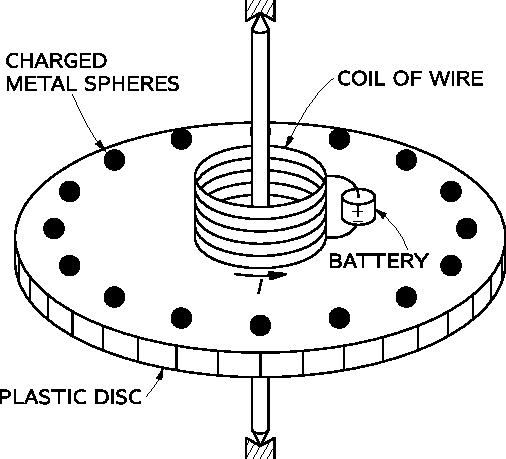
\includegraphics[width=0.8\linewidth]{fyz_fig336.pdf}
    \caption{Bude se kotouč otáčet, když přerušíme proud \(I\)?
             (\cite[s.~300]{Feynman02}).}
    \label{fyz:fig336}
  \end{figure}
  kružnic soustředěných s osou. Nabité kuličky na obvodu kotouče pocítí tečnou elektrickou sílu. 
  Tato elektrická síla má stejný smysl pro všechny náboje, a proto vyvolá otáčivý moment působící 
  na kotouč. Pod vlivem těchto argumentů bychom čekali, že zánikem proudu v solenoidu by se měl 
  kotouč začít otáčet. Známe-li moment setrvačnosti disku, proud tekoucí solenoidem a náboje
  na kuličkách, můžeme vypočítat výslednou úhlovou rychlost.
  
  Můžeme však argumentovati jinak. Použijeme-li princip zachování momentu hybnosti, můžeme 
  prohlásit, že moment hybnosti kotouče se vším zařízením byl na počátku nulový, a proto by měl 
  nulový zůstat. Po přerušení proudu by nemělo dojít k žádnému otáčení. Která argumentace je 
  správná? Bude nebo nebude kotouč rotovat? Na tuto otázku byste měli po úvaze odpovědět vy.
  
  Bude třeba upozornit, že správná odpověď nezávisí na nějakém nepodstatném prvku, jakým je 
  například asymetrická poloha baterie. Můžeme si vlastně představit ideální situaci, kdy je 
  solenoid sestrojen ze supravodivého drátu, a tím protéká proud. Potom, když jsme kotouč opatrně 
  usadili, teplotu solenoidu nepatrně zvýšíme. Když teplota dosáhne hodnoty, při níž supravodivost 
  přechází na normální vodivost, poklesne proud v solenoidu na nulu v důsledku odporu vodiče. Tak 
  jako předtím klesne magnetický tok k nule a kolem osy vznikne elektrické pole. Je nutné říci, že 
  řešení není jednoduché, ale není v něm žádný trik. Najdeme-li řešení, objevíme důležitý princip 
  elektromagnetizmu.
  
\section{Generátor střídavého proudu}\label{fyz:IIchapXVIIsecV}
  Ve zbývající části této kapitoly použijeme principy článku \ref{fyz:IIchapXVIIsecI} k analýze 
  jevů, o nichž jsme diskutovali v kapitole \ref{fyz:IIchapXVI}. Nejdříve si podrobněji všimneme 
  generátoru střídavého proudu. Základem takového generátoru je vodivá cívka otáčející se v 
  homogenním magnetickém poli. Stejného výsledku dosáhneme i tehdy, když máme nepohyblivou cívku v 
  magnetickém poli, jehož směr se otáčí tak, jak bylo popsáno v předcházející kapitole. Budeme však 
  uvažovat jen první případ. Předpokládejme, že máme kruhovou vodivou cívku, jež se může otáčet 
  kolem osy procházející jedním z jejích průměrů. Tuto cívku umístíme do magnetického pole, které 
  je kolmé k ose otáčení tak, jak znázorňuje obr.\ref{fyz:fig337}. Dále si představme, že oba konce 
  cívky jsou připojeny k vnějšímu obvodu pomocí nějakých kluzných kontaktů. V důsledku otáčení 
  cívky se bude měnit magnetický tok, který jí prochází. V obvodu cívky se proto projeví emn. Nechť 
  je \(S\) plocha cívky a \(\vartheta\) úhel mezi magnetickým polem a normálou k rovině cívky. Pak 
  je tok cívkou roven
  \begin{equation}\label{fyz:eq390}
    BS\cos\vartheta.
  \end{equation}
  
  \begin{figure}[ht!]  %\ref{fyz:fig337}
    \centering
    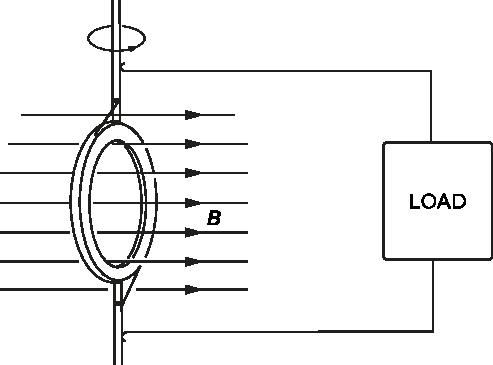
\includegraphics[width=0.8\linewidth]{fyz_fig337.pdf}
    \caption{Vodivá cívka otáčející se v homogenním magnetickém poli - základní myšlenka generátoru 
             střídavého proudu.
             (\cite[s.~301]{Feynman02}).}
    \label{fyz:fig337}
  \end{figure}
  Otáčí-li se cívka konstantní úhlovou rychlostí \(\omega\), mění se \(\vartheta\) s časem podle 
  závislosti \(\vartheta = \omega t\). Každý závit cívky bude mít emn rovno rychlosti změny tohoto 
  toku. Má-li cívka \(N\) závitů, bude celkové emn \(N\)-krát větší, takž
  \begin{equation}\label{fyz:eq391}
    \mathscr{E} = - N\der{ }{t}(BS\cos\omega t)= NBS\sin\omega t.
  \end{equation}
  
  Vyvedeme-li vodiče z generátoru na místo, které je dost daleko od otáčející se cívky, takže 
  magnetické pole tam je nulové, nebo se alespoň s časem nemění, bude rotace \(\vec{E}\) v této 
  oblasti nulová a můžeme definovat potenciál. Neodebíráme-li z generátoru žádný proud, bude 
  potenciálový rozdíl \(U\) mezi těmi dvěma vodiči roven emn otáčející se cívky, tj.
  \begin{equation}\label{fyz:eq392}
    U = NBS\omega\sin\omega t)= U_0\sin\omega t.
  \end{equation}
  
  Potenciálový rozdíl mezi vodiči se mění jako \(\sin\omega t\). Takto se měnící rozdíl potenciálů 
  se nazývá střídavé napětí.
  
  Protože mezi vodiči je elektrické pole, musí být elektricky nabité. Je jasné, že emn generátoru 
  vtlačuje nadbytečné náboje do vodiče, pokud od nich pocházející pole není dost silné k vyrovnání 
  indukční síly. Podíváme-li se na generátor zvenku, chovají se oba vodiče tak, jako kdyby byly 
  elektrostaticky nabité na potenciální rozdíl \(U\) a jako kdyby se náboj měnil s časem tak, že by 
  dával střídavý potenciálový rozdíl. Oproti elektrostatice je tu ještě jeden rozdíl. Připojíme-li 
  generátor  k vnějšímu obvodu, který umožňuje protékání proudu, zjistíme, že emm nedovoluje vybití 
  vodičů, ale pokračuje v dodávání náboje, dokud je odebírán proud. Děje se to takovým způsobem, že 
  emn se vždy snaží udržet stejný potenciálový rozdíl vodičů. Je-li generátor připojen k obvodu, 
  jehož celkový odpor je \(R\), bude proud protékající obvodem přímo úměrný emn generátoru a 
  nepřímo úměrný \(R\). Protože emn má sinusový časový průběh, bude jej mít i proud. Vzniká 
  střídavý proud
  \begin{equation}\label{fyz:eq393}
    I = \frac{\mathscr{E}}{R}= \frac{U_0}{R}\sin\omega t.
  \end{equation}
  Schématicky je takový obvod znázorněn na obr. \ref{fyz:fig338}.

  \begin{figure}[ht!]  %\ref{fyz:fig338}
    \centering
    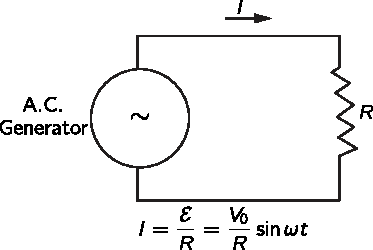
\includegraphics[width=0.6\linewidth]{fyz_fig338.pdf}
    \caption{Obvod s generátorem střídavého proudu a odporem 
             (\cite[s.~302]{Feynman02}).}
    \label{fyz:fig338}
  \end{figure}
  
  Také je vidět, že emn určuje, kolik energie dodává generátor. Každý náboj ve vodiči dostává za 
  jednotku času energii \(\vec{F}\cdot\vec{v}\), kde \(\vec{F}\) je síla působící na náboj a 
  \(\vec{v}\) je jeho rychlost. Nechť je počet nábojů pohybujících se v délkové jednotce vodiče 
  roven \(n\); výkon dodávaný do elementu \(ds\) vodiče je pak roven
  \begin{equation}\label{fyz:eq394}
    \vec{F}\cdot\vec{v}n\dd{s}.
  \end{equation}
  Ve vodiči směřuje \(\vec{v}\) vždy podél \(\dd{\vec{s}}\), a proto lze výkon vyjádřit ve tvaru
  \begin{equation}\label{fyz:eq395}
    nv\vec{F}\cdot\dd{\vec{s}}.
  \end{equation}
  Celkový výkon dodávaný do obvodu je pak integrálem tohoto výrazu podél celé smyčky:
  \begin{equation}\label{fyz:eq396}
    \text{výkom} = \oint nv\vec{F}\cdot\dd{\vec{s}}.
  \end{equation}
  Připomeňme, že \(qnv\) je proud \(I\) a že emn je definováno jako integrál \(F/q\) po celém 
  obvodu. Tak dostaneme výsledek 
  \begin{equation}\label{fyz:eq397}
    \text{výkon dodávaný generátorem} = \mathscr{E}I.
  \end{equation}
  
  Teče-li cívkou generátoru proud, budou na ni působit i mechanické síly. Už víme, že moment sil 
  působící na cívku je úměrný jejímu magnetickému momentu, magnetické indukci \(B\) a sinu úhlu 
  mezi těmito veličinami. Magnetický moment je součin plochy cívky a proudu, který jí protéká. 
  Proto moment sil vyjádříme takto:
  \begin{equation}\label{fyz:eq398}
    \tau = NISB\sin\vartheta.
  \end{equation}
  Rychlost s níž se musí konat mechanická práce, aby se cívka otáčela, je součin úhlové frekvence 
  \(\omega\) a momentu hybnosti
  \begin{equation}\label{fyz:eq399}
    \der{W}{t} = \omega\tau = \omega NISB\sin\vartheta.
  \end{equation}
  Porovnáváme-li tuto rovnici s rovnicí (\ref{fyz:eq391}) vidíme, že rychlost, s jakou musí být 
  konána mechanická práce, aby se cívka otáčela proti magnetickým silám, je rovna právě 
  \(\mathscr{E}I\), tedy rychlosti, sníž je dodávána elektrická energie emngenerátoru. Všechna 
  mechanická energie spotřebovaná generátorem se objevuje jako elektrická energie v obvodu.
 
  Jako další příklad proudů a sil podmíněných indukovaným emm si všimněme, co se odehrává
  v zařízení popsaném v kapitole \ref{fyz:IIchapXVIIsecI} a znázorněném na obr. \ref{fyz:fig332}. 
  Máme tam dva rovnoběžné vodiče, na jednom konci pevně propojené tak jako písmeno U a na druhém 
  konci přeložené kluznou tyčkou. To vše je v homogenním magnetickém poli kolmém k rovině 
  rovnoběžných vodičů. Předpokládejme, že „spodek“ písmene U (na levé straně obrázku) je z 
  materiálu, který má velký odpor, zatímco dva boční vodiče jsou z dobře vodivého materiálu, jako 
  např. měď. Pak se nemusíme znepokojovat změnami odporu v obvodu při pohybu kluzné tyčky. Tak jako 
  předtím pro emn v obvodu platí
  \begin{equation}\label{fyz:eq400}
    \mathscr{E} = vBw.
  \end{equation}
  Proud v obvodu je přímo úměrný tomuto emn a nepřímo úměrný odporu obvodu
  \begin{equation}\label{fyz:eq401}
    I = \frac{\mathscr{E}}{R} = \frac{vBw}{R}.
  \end{equation}
  
  V důsledku tohoto proudu bude na kluznou tyčku působit magnetická síla, která je úměrná délce 
  tyčky, magnetickému poli a proudu, který okruhem protéká, takže
  \begin{equation}\label{fyz:eq402}
    F = BIw.
  \end{equation}
  Dosadíme-li za \(I\) z rovnice (\ref{fyz:eq401}), dostaneme pro sílu vyjádření
  
  Vidíme, že síla je úměrná rychlosti pohybu tyčky. Snadno zjistíme, že směr síly je opačný ke 
  směru rychlosti. Taková síla „úměrná rychlosti“, podobná viskózní síle, se objevuje vždy, když 
  vodiče pohybující se v magnetickém poli vytvářejí indukované proudy. Vířivé proudy, o nichž jsme 
  hovořili v předcházející kapitole, také vyvolávají síly úměrné rychlosti vodiče, ačkoli v těchto 
  případech bývá rozdělení proudů složité a analýza problémů obtížná. 
  
  Při konstrukci mechanických systémů se často s výhodou využívají tlumivé síly úměrné rychlosti. 
  Jeden z nejvhodnějších způsobů získání takových sil závislých na rychlosti je využití vířivých 
  proudů. Příklad aplikace takové síly najdete v obyčejném domácím wattmetru. Je v něm tenký 
  hliníkový kotouč, který rotuje mezi póly permanentního magnetu. Tento kotouč je poháněn malým 
  elektromotorem, jehož moment síly je úměrný výkonu spotřebovanému v elektrických obvodech 
  domácnosti. Působením vířivých proudů v kotouči vzniká síla odporu úměrná rychlosti. V rovnováze 
  proto bude rychlost úměrná rychlosti spotřeby elektrické energie. Pomocí počítače připojeného k 
  rotujícímu kotouči získáváme údaj o počtu otáček, které kotouč uskutečnil. Tento údaj určuje 
  celkovou spotřebovanou energii, tj. počet spotřebovaných watthodin. 
  
  Ze vztahu (\ref{fyz:eq402}) je vidět, že síla indukovaných proudů, tj. síla všech vířivých 
  proudů, je nepřímo úměrná odporu. Síla bude tím větší, čím větší je vodivost materiálu. Příčina 
  spočívá v tom, že při malém odporu vytváří emm větší proud a větší proudy dávají větší mechanické 
  síly. 
  
  Z našich vztahů lze vypozorovat i to, že elektrická energie dodaná odporu v obvodu je rovna 
  součinu \(\mathscr{E}I\). Rychlost, s níž je vykonávána práce při pohybu kluzné tyčky, je rovna 
  součinu rychlosti tyčky a síly, která na ni působí. Vyjádříme-li sílu pomocí vztahu 
  (\ref{fyz:eq401}), dostaneme pro rychlost konání práce výraz
  \begin{equation}\label{fyz:eq403}
    \der{W}{t} = \frac{B^2w^2}{R}.
  \end{equation}  
  Tento výraz je opravdu roven součinu \(\mathscr{E}I\), který bychom dostali ze vztahů 
  (\ref{fyz:eq400}) a (\ref{fyz:eq401}). Mechanická práce se opět objevuje jako elektrická energie.
  
\section{Vzájemná indukčnost}\label{fyz:IIchapXVIIsecVI}
  Nyní bychom měli uvažovat takovou situaci, kdy jsou vodivé cívky pevné, ale mění se magnetická 
  pole. Když jsme popisovali vytváření magnetických polí proudy, uvažovali jsme pouze případ 
  stacionárních proudů. Pokud se však proudy budou měnit pomalu, bude magnetické pole v každém 
  okamžiku téměř stejné jako magnetické pole ustáleného proudu. V této části budeme předpokládat, 
  že proudy se mění vždy dostatečně pomalu, takže předcházející tvrzení je pravdivé.
  
  \begin{figure}[ht!]  %\ref{fyz:fig339}
    \centering
    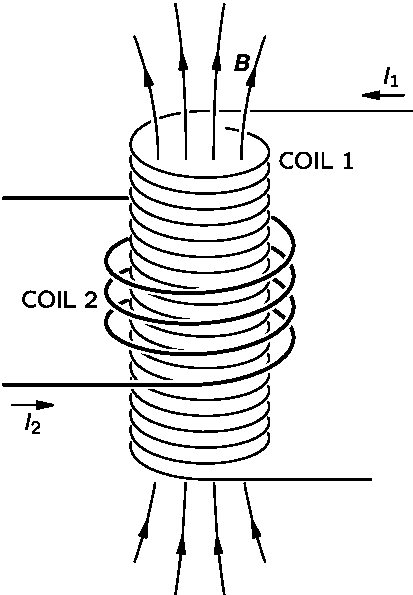
\includegraphics[width=0.6\linewidth]{fyz_fig339.pdf}
    \caption{Proud tekoucí cívkou \(1\) vytváří magnetické pole procházející průřezem cívky \(2\)
             (\cite[s.~304]{Feynman02}).}
    \label{fyz:fig339}
  \end{figure}
  
  Na obr. \ref{fyz:fig339} je znázorněno seskupení dvou cívek, pomocí něhož lze demonstrovat 
  základní jevy, na nichž je založena činnost \textbf{transformátoru}. Cívka \(1\) se skládá z 
  vodivého drátu navinutého ve tvaru dlouhého solenoidu. Kolem této cívky - a izolovaně od ní - je 
  navinuta cívka \(2\), skládající se z několika závitů drátu. Víme, že v cívce \(1\) se objeví 
  magnetické pole, poteče-li jí proud. Toto magnetické pole prochází i cívkou \(2\). Mění-li se 
  proud v cívce \(1\), bude se měnit i magnetický tok a v cívce \(2\) se objeví indukované emm. 
  Toto indukované emn nyní vypočítáme.
  
  V části \ref{fyz:IIchapXIIIsecV} jsme poznali, že magnetické pole uvnitř dlouhého solenoidu je 
  homogenní a má
  \begin{equation}\label{fyz:eq404}
    B = \frac{1}{\varepsilon_0c^2}\frac{N_1I_1}{l}.
  \end{equation}
  kde \(N_1\) je počet závitů cívky \(1\), \(I_1\) je proud tekoucí touto cívkou a \(l\) je její 
  délka. Nechť příčný řez cívkou \(1\) má plochu \(S\). Tok pole \(\vec{B}\) je pak roven součinu 
  jeho velikosti a plochy \(S\). Má-li cívka \(2\) \(N_2\) závitů, prochází tento tok cívkou 
  \(N_2\)-krát. Proto lze emn v cívce \(2\) vyjádřit vztahem
  \begin{equation}\label{fyz:eq405}
    \mathscr{E}_2 = -N_2S\der{B}{t}.
  \end{equation}
  Jedinou veličinou ve vztahu (\ref{fyz:eq404}), která se s časem mění, je \(I_1\). Proto pro emn 
  platí
  \begin{equation}\label{fyz:eq406}
    \mathscr{E}_2 = \frac{N_1N_2S}{\varepsilon_0c^2l}\der{I_1}{t}.
  \end{equation}
  
  Vidíme, že emn v cívce \(2\) je úměrné rychlosti změny proudu v cívce \(1\). Konstanta úměrnosti, 
  která je vlastně geometrickým faktorem těchto cívek, se nazývá \textbf{vzájemná indukčnost} a 
  obvykle se označuje \(M_{12}\)
  \begin{equation}\label{fyz:eq407}
    \mathscr{E}_2 = M_{21}\der{I_1}{t}.
  \end{equation}
  
  Nyní předpokládejme, že bychom měli vést proud cívkou \(2\) a chtěli bychom vědět, jaké je emn v 
  cívce \(1\). Vypočítali bychom magnetické pole, které je všude úměrné proudu \(I_2\). Tok cívkou 
  \(1\) by závisel na geometrii, ale byl by úměrný proudu \(I_2\). Emn v cívce \(1\) by proto bylo 
  opět úměrné \(\der{I_2}{t}\) takže
  \begin{equation}\label{fyz:eq408}
    \mathscr{E}_1 = M_{12}\der{I_2}{t}.
  \end{equation}
  Výpočet \(M_{12}\) by byl těžší než výpočet \(M_{21}\), který jsme uvedli. Nebudeme jej však 
  dělat, neboť ještě v této kapitole ukážeme, že \(M_{12}\) musí být rovno \(M_{21}\).
  
  Protože pole \emph{libovolné} cívky je úměrné proudu, který jí protéká, dostali bychom podobný 
  výsledek pro libovolné dvě vodivé cívky. Rovnice (\ref{fyz:eq407}) a (\ref{fyz:eq408}) by měly 
  tentýž tvar, jen konstanty \(M_{21}\) a \(M_{12}\) by byly jiné. Jejich hodnoty by závisely na 
  tvarech cívek a najejich vzájemné poloze.
  
  \begin{figure}[ht!]  %\ref{fyz:fig340}
    \centering
    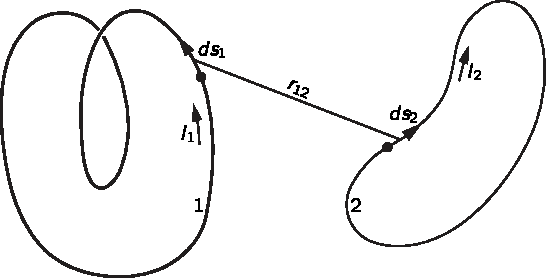
\includegraphics[width=0.8\linewidth]{fyz_fig340.pdf}
    \caption{Dvě libovolné cívky mají zvájemnou indukčnost \(M\) úměrnou integrálu z 
            \(\dd{\vec{s}_1}\cdot\dd{\vec{s}_2}/r_{12}\)
             (\cite[s.~305]{Feynman02}).}
    \label{fyz:fig340}
  \end{figure}

  Předpokládejme, že bychom chtěli najít vzájemnou indukčnost mezi dvěma libovolnými cívkami, např. 
  takovými, jaké znázorňuje obr. \ref{fyz:fig340}. Víme, že obecný výraz pro emn v 
  cívce \(1\) lze zapsat ve tvaru
  \begin{equation}\label{fyz:eq409}
    \mathscr{E}_1 = - \der{ }{t}\int_{(1)}\vec{B}\cdot\vec{n}\dd{S},
  \end{equation}
  kde \(\vec{B}\) je magnetické pole a integrál je třeba brát po ploše ohraničené obvodem \(1\). 
  V článku \ref{fyz:IIchapXIVsecI} jsme už viděli, že takový plošný integrál z \(\vec{B}\) lze 
  vyjádřit pomocí křivkového integrálu vektorového potenciálu. Konkrétně
  \begin{equation}\label{fyz:eq410}
    \int_{(1)}\vec{B}\cdot\vec{n}\dd{S} = \oint_{(1)}\vec{A}\cdot\dd{\vec{s_1}},
  \end{equation}
  kde \(\vec{A}\) představuje vektorový potenciál a \(\dd{\vec{s}}\) je element obvodu \(1\). 
  Křivkový integrál je brán podél obvodu \(1\). Emm v cívce \(1\) lze pak vyjádřit ve tvaru
  \begin{equation}\label{fyz:eq411}
    \mathscr{E}_1 = -\der{ }{t}\oint_{(1)}\vec{A}\cdot\dd{\vec{s_1}},
  \end{equation}
  
  Nyní předpokládejme, že vektorový potenciál v obvodu \(1\) pochází od proudů v obvodu \(2\). 
  Proto je možné jej vyjádřit jako křivkový integrál podél obvodu \(2\)
  \begin{equation}\label{fyz:eq412}
    \vec{A} = \frac{1}{4\pi\varepsilon_0c^2}\oint_{(2)}\frac{I_2\dd{\vec{s_2}}}{r_{12}},
  \end{equation}
  kde \(I_2\) je proud v obvodu \(2\) a \(r_{12}\) je vzdálenost od elementu obvodu 
  \(\dd\vec{s_2}\), k tomu bodu v obvodu \(1\), ve kterém určujeme vektorový potenciál (obr. 
  \ref{fyz:fig340}). Zkombinujeme-li vztahy (\ref{fyz:eq411}) a (\ref{fyz:eq412}), můžeme emn v 
  obvodu \(1\) vyjádřit jako dvojitý křivkový integrál
  \begin{equation}\label{fyz:eq413}
    \mathscr{E}_1 = - \frac{1}{4\pi\varepsilon_0c^2}\der{ }{t}
                    \oint_{(1)}\oint_{(2)}\frac{I_2\dd{\vec{s_2}}}{r_{12}}\cdot\dd{\vec{s_1}}.
  \end{equation}
  V tomto vztahu se všechny integrály berou podél nehybných obvodů. Jedinou proměnnou veličinou je 
  proud \(I_2\), který nezávisí na integračních proměnných. Můžeme jej proto dát před
  integrály. Pro emn pak dostaneme 
  \begin{equation*}
    \mathscr{E}_1 = M_{12}\der{I_2}{t},
  \end{equation*}
  kde \(M_{12}\) je koeficient vyjádřený vztahem
  \begin{equation}\label{fyz:eq414}
    M_{12} = - \frac{1}{4\pi\varepsilon_0c^2}\der{ }{t}
             \oint_{(1)}\oint_{(2)}\frac{\dd{\vec{s_1}}\cdot\dd{\vec{s_2}}}{r_{12}}.
  \end{equation}
  Z tohoto vyjádření je zřejmé, že \(M_{12}\)  závisí pouze na geometrii obvodu. Závisí na jisté 
  střední vzdálenosti těchto obvodů, přičemž s největší váhou se na vystředování účastní paralelní 
  úseky obou cívek. Naši rovnici lze použít k výpočtu vzájemné indukčnosti libovolných dvou obvodů
  jakéhokoliv tvaru. Také je vidět, že integrál pro \(M_{12}\)  je shodný s integrálem pro 
  \(M_{21}\) . Tak jsme dokázali, že tyto koeficienty jsou shodné. Máme-li soustavu pouze dvou 
  cívek, používáme často místo symbolů \(M_{12}\) a \(M_{21}\)  pouze symbol \(M\) a nazýváme jej 
  pouze \textbf{vzájemnou indukčností}:
  \begin{equation*}
    M_{12} =  M_{21} = M.
  \end{equation*}
  
\section{Samoindukčnost}\label{fyz:IIchapXVIIsecVII}
  Při zkoumání indukovaných elektromotorických napětí ve dvou cívkách znázorněných na obr. 
  \ref{fyz:fig339}, resp. \ref{fyz:fig340} jsme uvažovali jen případ, kdy proud tekl pouze jednou s 
  cívek. Potečou-li proudy oběma cívkami současně, bude magnetický tok procházející každou z cívek 
  součtem dvou toků, jež by existovaly odděleně, neboť pro magnetická pole platí zákon superpozice. 
  Emn v každé cívce proto bude úměrné nejen změně proudu v cívce druhé, ale i změně proudu v ní 
  samé. Pro celkové emn v cívce \(2\) tedy platí\footnote{Znaménko \(M_{12}\) a  \(M_{21}\) v 
  \ref{fyz:eq415} a \ref{fyz:eq416} závisí na volné výběru kladného směru proudu v obou cívkách},
  \begin{equation}\label{fyz:eq415}
    \mathscr{E}_2 = M_{21}\der{I_1}{t} + M_{22}\der{I_2}{t}.
  \end{equation}
  Podobně bude emn v cívce \(1\) záviset nejen na měnícím se proudu v cívce \(2\), ale i na měnícím 
  se proudu v ní samé.
  \begin{equation}\label{fyz:eq416}
    \mathscr{E}_1 = M_{12}\der{I_2}{t} + M_{11}\der{I_1}{t}.
  \end{equation}
  Koeficienty \(M_{22}\) a \(M_{11}\) jsou vždy záporné. Obvykle je zapisujeme jako 
  \begin{equation}\label{fyz:eq417}
    M_{11} = -L_1,\quad  M_{22} = - L_2,
  \end{equation}
  kde \(L_1\) a \(L_2\) nazýváme \textbf{samoindukčnost cívek}. 
  
  \begin{figure}[hb!]
    \centering
    \subcaptionbox{\label{fyz:fig341a}}{\luafigure[0.3]{fyz_fig341a.pdf}}         
    \subcaptionbox{\label{fyz:fig341b}}{\luafigure[0.6]{fyz_fig341b.pdf}}
    \caption{a) Obvod se zdrojem napětí a s indukčností, b) Analogický mechanický systém
             (\cite[s.~307]{Feynman02}).}
    \label{fyz:fig341}
  \end{figure}
  
  Emm samoindukce bude, samozřejmě, existovat i tehdy, když máme jen jednu cívku. Libovolná cívka 
  má sama indukčnost \(L\). Emm bude úměrné rychlosti změny proudu vní. V případě samostatné cívky 
  se obvykle dohodneme na tom, že emn a proud považujeme za kladné, mají-li shodný směr. Pak můžeme 
  pro emn samotné cívky psát
  \begin{equation}\label{fyz:eq418}
    \mathscr{E} = - L\der{I}{t}.
  \end{equation}
  Záporné znaménko svědčí o tom, že emn působí proti změnám proudu a toto emn se často nazývá 
  „zpětné emn“.
  
  Protože v každé cívce existuje samoindukce, která působí proti proudovým změnám, bude proud v 
  cívce vykazovat určitý druh setrvačnosti. Skutečně, chceme-li změnit proud v cívce, musíme 
  překonat tuto setrvačnost připojením cívky k nějakému vnějšímu zdroji napětí, jakým je baterie 
  nebo generátor (to je schématicky znázorněno na obr. \ref{fyz:fig341a}). V takovémto obvodě 
  závisí proud \(I\) na napětí \(U\) podle vztahu
  \begin{equation}\label{fyz:eq419}
    U = - L\der{I}{t}.
  \end{equation}
  
  Tento vztah má tvar Newtonova pohybového zákona pro částici pohybující se v jednom směru. Můžeme 
  ji zkoumat na základě principu, že „stejné rovnice mají stejná řešení“. Přiřadíme-li tedy vnější 
  napětí \(U\) působící síle \(F\) a proudu \(I\) v cívce přiřadíme rychlosti \(v\) částice, bude 
  potom indukčnost cívky \(L\) odpovídat hmotnosti \(m\) částice (obr. 
  \ref{fyz:fig341b})\footnote{Mimochodem, toto není jediný způsob, kterým je možné zavést 
  souvislost mezi mechanickými a elektrickými Veličinami.}. Tímto způsobem je sestavena tab. 
  \ref{fyz:tab009}, která vystihuje souvislost mezi mechanickými a elektrickými veličinami.

  \begin{table}[ht!] %\ref{fyz:tab009}
    \centering
    \renewcommand{\arraystretch}{1.4}
    \begin{tabular}{c|c}
           \hline \textbf{částice}  & \textbf{Cívka}                            \\ \hline
                       \(F\) (síla) & \(U\) (napětí, rozdíl potenciálů)         \\
                \(v\) (rychlost)    & \(I\) (proud)                             \\
                \(x\) (posunutí)    & \(q\) (náboj)                             \\
                \(F = m\der{v}{t}\) & \(U = L\der{I}{t}\)                       \\
                \(mv\) (hybnost)    & \(LI\)                                    \\
       \(\frac{1}{2}mv^2\) (kinetická enerige) & \(\frac{1}{2}LI^2\) (magnetická enerige)     \\
       \hline 
    \end{tabular}
    \caption{(\cite[s.~308]{Feynman01})}
    \label{fyz:tab009}
  \end{table}
    
\section{Indukčnost a magnetická energie}\label{fyz:IIchapXVIIsecVIII}
  V analogii, kterou jsme zavedli v předcházející části, bychom mohli pokračovat dále. Tak bychom 
  přišli k poznatku, že mechanické hybnosti \(p=mv\), jejíž rychlost změny je rovna působící síle, 
  by měla odpovídat analogická veličina rovna \(LI\), jejíž rychlost změny je \(U\). Samozřejmě, že 
  nemáme právo říkat, že \(LI\) je skutečná hybnost obvodu (ona jí totiž ani není). Celý obvod může
  být nehybný, a proto ani hybnost nemá. Veličina \(LI\) je pouze veličině \(mv\) analogická v tom 
  smyslu, že vyhovuje podobným rovnicím. Stejným způsobem odpovídá kinetické energii 
  \(\frac{1}{2}mv^2\) analogická veličina \(\frac{1}{2}LI^2\). Zde nás však čeká překvapení. Tato 
  veličina \(\frac{1}{2}LI^2\) je skutečně energie i v elektrickém případě. Je tomu tak, protože 
  rychlost konání práce na indukčnosti je rovna \(UI\) a v mechanickém systému je rovna \(Fv\) - 
  což je odpovídající veličina. Proto v případě energie jde nejen o matematickou korespondenci 
  veličin, ale mají také týž fyzikální význam. 

  Podívejme se na to podrobněji. Ve vztahu (\ref{fyz:eq397}) jsme viděli, že rychlost konání 
  elektrické práce indukovanými silami je rovna součinu elektromotorického napětí a proudu
  \begin{equation*}
    \der{W_{ind}}{t} = \mathscr{E}I.
  \end{equation*}
  Nahradíme-li ve shodě se vztahem (\ref{fyz:eq418}) \(\mathscr{E}\) výrazem, v němž vystupuje 
  proud, dostaneme
  \begin{equation}\label{fyz:eq420}
    \der{W_{ind}}{t} = -LI\der{I}{t}.
  \end{equation}
  Zintegrujeme-li tuto rovnici, zjistíme, že energie z vnějšího zdroje, potřebná k překonání emn 
  při samoindukci po dobu nárůstu proudu\footnote{Zanedbáváme všechny tepelné ztráty energle 
  způsobené průchodem proudu odporem cívky. Takové ztráty vyžadují dodatečnou energii od zdroje, 
  ale nemění energii, která je transformována indukčností.} (jež musí být rovna nahromaděné energii 
  \(W\)) je rovna
  \begin{equation}\label{fyz:eq421}
     - W_{ind} = W = \frac{1}{2}LI^2.
  \end{equation}
  Proto je energie nahromaděná v indukčnosti rovna \(\frac{1}{2}LI^2\).
  
  Použijeme-li tyto argumenty na případ dvou cívek, např. takových, jaké znázorňuje obr. 
  \ref{fyz:fig339} nebo \ref{fyz:fig340}, můžeme ukázat, že celková elektrická energie systému je 
  dána vztahem
  \begin{equation}\label{fyz:eq422}
    W = \frac{1}{2}L_1I_1^2 + \frac{1}{2}L_2I_2^2 + MI_1I_2.
  \end{equation}
  Kdybychom vycházeli ze situace, že \(I = 0\) v obou cívkách, mohli bychom nejprve zapnout proud 
  \(I_1\) v cívce \(1\) při nezměněném \(I_2 = 0\). Vykonaná práce je pak rovna 
  \(\frac{1}{2}L_1I_1^2\). Zapneme-li potom \(I_2\) , nekonáme pouze práci \(\frac{1}{2}L_2I_2^2\) 
  proti emn obvodu \(2\), ale i dodatečné množství práce \(MI_1I_2\), které je integrálem emn 
  [\(M(dI_2/dt)\)] v obvodu \(1\) násobeným nyní už \emph{konstantním} proudem \(I_1\) v tomto 
  obvodu.
  
  Hledejme sílu působící mezi libovolnými dvěma cívkami, jimiž tečou proudy \(I_1\) a \(I_2\). Dalo 
  by se čekat, že bude možné použít princip virtuální práce a provést variaci energie vyjádřené 
  vztahem (\ref{fyz:eq422}). Musíme však mít na zřeteli, že při změně vzájemné polohy cívek je 
  vzájemná indukčnost \(M\) jedinou proměnnou veličinou. Pak bychom mohli psát rovnici virtuální 
  práce ve tvaru
  \begin{equation}\label{fyz:eq423}
    -F\Delta x = \Delta W = I_1I_2\Delta M \quad (\text{nesprávně}).
  \end{equation}

  Tato rovnice je nesprávná, neboť zahrnuje (jak už jsme poznali dříve) pouze změny energie dvou 
  cívek, a ne změnu energie zdrojů, které udržují proudy \(I_1\) a \(I_2\), na stálých hodnotách. 
  Už víme, že tyto zdroje musí dodávat energii ke kompenzaci indukovaných emn v cívkách, když se 
  tyto pohybují. Chceme-li správně aplikovat princip virtuální práce, musíme zahrnout i tyto 
  energie. Už jsme však viděli, že postup je možné zkrátit tehdy, když si při použití principu 
  virtuální práce uvědomíme, že celková energie je vlastně mechanická energie \(W_{mech}\) s 
  opačným znaménkem. Proto můžeme pro sílu psát
  \begin{equation}\label{fyz:eq424}
    -F\Delta x = \Delta W_{mech} = -\Delta W.
  \end{equation}
  Pak pro sílu mezi dvěma cívkami platí
  \begin{equation*}
    F\Delta x = I_1I_2\Delta M.
  \end{equation*}
  
  Rovnici (\ref{fyz:eq422}) pro energii systému dvou cívek využijeme k tomu, abychom odvodili 
  zajímavou nerovnost mezi vzájemnou indukčností \(M\) a samoindukčnostmi \(L_1\) a \(L_2\) dvou 
  cívek. Je jasné, že energie dvou cívek musí být kladná. Začneme-li s nulovými proudy v cívkách a 
  tyto proudy pak zvětšíme na nějakou hodnotu, dodáme tím energii našemu systému. V opačném případě 
  by proudy samovolně rostly a odevzdávaly energii okolnímu světu, což je nepravděpodobné. Naši 
  rovnici pro energii (\ref{fyz:eq422}) můžeme vyjádřit v ekvivalentním tvaru
  \begin{equation}\label{fyz:eq425}
    W = \frac{1}{2}L_1\left(I_1+\frac{M}{L_1}I_2\right)^2 + 
        \frac{1}{2}\left(L_2-\frac{M^2}{L_1}\right)I_2^2.
  \end{equation}
  Je to prostá algebraická transformace. Tato veličina musí být vždy kladná při libovolných 
  hodnotách \(I_1\) a \(I_2\). Musí být kladná i tehdy, když \(I_2\), nabývá hodnoty
  \begin{equation}\label{fyz:eq426}
    I_2 = - \frac{L_1}{M}I_1.
  \end{equation}
  Pro takový proud je však první člen v rovnici (\ref{fyz:eq426}) nulový. Má-li být energie kladná, 
  musí být druhý člen v rovnici (\ref{fyz:eq425}) větší než nula. Tak dostaneme podmínku
  \begin{equation}\label{fyz:eq427}
    L_1L_2 >M^2.
  \end{equation}
  Dokázali jsme tedy obecné tvrzení, že hodnota vzájemné indukčnosti \(M\) dvou libovolných cívek
  je nevyhnutelně menší, nebo je rovna geometrickému průměru dvou indukčností. (Samotné \(M\) může 
  být kladné nebo záporné podle toho, jak byla vybrána znaménka proudů \(I_1\), \(I_2\)):
  \begin{equation}\label{fyz:eq428}
    \abs{M}\leq \sqrt{L_1L_2}.
  \end{equation}
  Vztah mezi \(M\) a samoindukčnostmi je obvykle zapisován ve tvaru
  \begin{equation}\label{fyz:eq429}
    M =  k\sqrt{L_1L_2}.
  \end{equation}
  Konstanta \(k\) se nazývá \textbf{vazbový koeficient}. Prochází-li většina magnetického toku z 
  jedné cívky druhou cívkou, bude se koeficient vazby blížit jedné; říkáme, že cívky jsou těsně 
  vázány. Jsou-li cívky od sebe velmi vzdálené, nebo je-li to zařízeno tak, že vzájemný průnik 
  jejich toků je velmi malý, bude se vazbový koeficient blížit nule a vzájemná indukčnost bude 
  velmi malá. 
  
  Pro výpočet vzájemné indukčnosti dvou cívek jsme uvedli vztah (\ref{fyz:eq414}), který 
  představuje dvojitý křivkový integrál podél dvou obvodů. Zdálo by se, že takový vztah lze použít 
  i pro výpočet samoindukce jedné cívky, počítáme-li oba integrály kolem téže cívky. To však není 
  možné, neboť při integrování kolem cívek se jmenovatel \(r_{12}\) integrandu blíží nule, jsou-li 
  dva křivkové elementy v jednom bodě. Takto získaná samoindukčnost je pak nekonečná. Příčina 
  spočívá v tom, že zmíněný vztah představuje aproximaci platnou jen tehdy, když jsou průřezy 
  vodičů dvou obvodů malé ve srovnání se vzdáleností mezi jednotlivými obvody. Tato aproximace je 
  prostě nevhodná pro samostatnou cívku. Je však pravda, že indukčnost samostatné cívky roste 
  logaritmicky k nekonečnu, volíme-li průměr vodiče stále menší a menší. 
  
  Musíme proto hledat způsob výpočtu samoindukce jedné cívky. Bude důležité zahrnout 
  \emph{rozložení} proudů ve vodičích, neboť rozměr vodiče se stává důležitým parametrem. Neměli 
  bychom se proto ptát na indukčnost „obvodu“, ale na indukčnost rozložení vodičů. Snad 
  nejjednodušším způsobem hledání této indukčnosti je využití magnetické energie. Už v článku 15.3 
  jsme našli výraz pro magnetickou energii rozložení stacionárních proudů:
  \begin{equation}\label{fyz:eq430}
    W = \frac{1}{2}\int\vec{j}\cdot\vec{A}\dd{V}.
  \end{equation}
  Známe-li rozdělení proudové hustoty \(\vec{j}\), můžeme vypočítat vektorový potenciál \(\vec{A}\) 
  a vypočtením integrálu ze vztahu (\ref{fyz:eq430}) určit energii. Tato energie je rovna 
  magnetické energii samoindukce \(\frac{1}{2}LI^2\). Porovnáním pak dostaneme vztah pro indukčnost
  \begin{equation}\label{fyz:eq431}
    L = \frac{1}{I^2}\int\vec{j}\cdot\vec{A}\dd{V}.
  \end{equation}
  Samozřejmě očekáváme, že indukčnost je číslo, které závisí jen na geometrii obvodu a ne na proudu 
  \(I\) v obvodu. Vztah (\ref{fyz:eq431}) však opravdu dává takový výsledek, neboť integrál v tomto 
  vztahuje úměrný druhé mocnině proudu - proud se tam jednou objevuje prostřednictvím \(\vec{j}\) a 
  podruhé prostřednictvím vektorového potenciálu \(\vec{A}\). Integrál dělený \(I^2\) pak bude 
  záviset na geometrii obvodu, a ne na proudu \(I\).
  
  Vztah (\ref{fyz:eq430}) pro energii rozložených proudů může být převeden do zcela odlišného 
  tvaru, který je pro výpočet někdy výhodnější. Později uvidíme, že tento tvar je důležitý proto, 
  že má obecnější platnost. V energetické rovnici (\ref{fyz:eq430}) souvisí \(\vec{A}\) i 
  \(\vec{j}\) s \(\vec{B}\), takže lze čekat, že energii je možné vyjádřit pomocí magnetického pole 
  - tak jako jsme dokázali dát do souvislosti elektrostatickou energii a elektrické pole. Začneme 
  tím, že \(\vec{j}\) nahradíme výrazem \(\varepsilon_0c^2\nabla\times\vec{B}\). Veličina 
  \(\vec{A}\) není jednoduše nahraditelná, neboť vztah \(\vec{B}=\nabla\times\vec{A}\) nelze 
  obrátit tak, aby vyjadřoval \(\vec{A}\) pomocí \(\vec{B}\). Můžeme však psát
  \begin{equation}\label{fyz:eq432}
    W = \frac{\varepsilon_0c^2}{2}\int(\nabla\times\vec{B})\cdot\vec{A}\dd{V}.
  \end{equation}
  
  Je zajímavé to, že při určitých omezeních lze tento integrál přepsat do tvaru
  \begin{equation}\label{fyz:eq433}
    W = \frac{\varepsilon_0c^2}{2}\int\vec{B}\cdot(\nabla\times\vec{A})\dd{V}.
  \end{equation}
  Abychom se o tom přesvědčili, zapíšeme podrobně jeden typický člen. Předpokládejme, že jsme vzali 
  člen \((\nabla\times\vec{B})_z\cdot\vec{A}_z\) který se vyskytuje v integrálu rovnice 
  (\ref{fyz:eq432}). Při zápisu pomocí složek máme
  \begin{equation*}
    \int(\pder{B_y}{x} - \pder{B_x}{y})A_z\dd{x}\dd{y}\dd{z}.
  \end{equation*}
  
  (Jsou tam, samozřejmě, dva další integrály stejného typu.) Nyní integrujeme první člen metodou 
  per partes. Tak dostaneme
  \begin{equation*}
    \int\pder{B_y}{x}A_z\dd{x} = B_yA_z - \int B_y\pder{A_z}{x}\dd{x}.
  \end{equation*}
  Předpokládejme, že náš systém, tj. zdroje a pole, je konečný, takže na velkých vzdálenostech se 
  všechna pole blíží nule. Integrujeme-li tedy přes celý prostor, dá člen \(B_yA_z\), v limitě 
  nulu. Zůstal nám jen člen s \(B_y(\pder{A_z}{x})\), který je zřejmě jednou částí 
  \(B_y\cdot(\nabla\times\vec{A})_y\), a tedy i \(\vec{B}\cdot(\nabla\times\vec{A})\). Kdybychom 
  vypočítali ostatních pět členů, viděli bychom, že rovnice (\ref{fyz:eq433}) je opravdu 
  ekvivalentní rovnici (\ref{fyz:eq432}). 
  
  Nyní však můžeme nahradit \((\nabla\times\vec{A})\) veličinou \(\vec{B}\) a dostaneme
  \begin{equation}\label{fyz:eq434}
    W = \frac{\varepsilon_0c^2}{2}\int\vec{B}\cdot\vec{B}\dd{V}.
  \end{equation}
  Energii magnetostatické situace jsme tedy vyjádřili pouze pomocí magnetického pole. Tento výraz 
  odpovídá výrazu, který jsme získali pro elektrostatickou energii
  \begin{equation}\label{fyz:eq435}
    W = \frac{\varepsilon_0}{2}\int\vec{E}\cdot\vec{E}\dd{V}.
  \end{equation}
  
  Jeden z důvodů, proč klademe důraz na tyto dva energetické vztahy, spočívá v tom, že jsou v 
  některých případech výhodnější než jiné vztahy. Důležité je však to, že v případě dynamických 
  polí (kdy \(\vec{E}\) a \(\vec{B}\) se s časem mění) zůstávají výrazy (\ref{fyz:eq434}) a 
  (\ref{fyz:eq435}) v platnosti, zatímco jiné vztahy, které jsme odvodili pro elektrostatickou nebo 
  magnetickou energii, už neplatí - jsou správné pouze pro statická pole.
  
  Známe-li magnetické pole \(\vec{B}\) jedné cívky, můžeme najít koeficient samoindukčnosti tak, že 
  výraz pro energii (\ref{fyz:eq434}) položíme roven výrazu \(\frac{1}{2}LI^2\). Zkoumejme, jaký 
  výsledek dostaneme pro koeficient samoindukčnosti dlouhého solenoidu. Už dříve jsme viděli, že 
  magnetické pole uvnitř solenoidu je konstantní a vně je \(\vec{B}\) nulové. Velikost pole uvnitř 
  solenoidu je rovna \(B = nI/\varepsilon_0c^2\), kde \(n\) je počet závitů na jednotku délky 
  vinutí a \(I\) je proud. Je-li poloměr cívky \(r\) a délka cívky \(l\) (\(l\) považujeme za velmi 
  dlouhé, takže můžeme zanedbat efekty na okrajích solenoidu, \(l\gg r\)), bude vnitřní objem \(\pi 
  r^2l\). Pro magnetickou energii proto platí
  \begin{equation*}
    W = \frac{\varepsilon_0c^2}{2}B^2\cdot(\text{objem}) = \frac{n^2I^2}{2\varepsilon_0c^2}\pi r^2l.
  \end{equation*}
  a tento výraz musí být roven i \(\frac{1}{2}LI^2\). Musí tedy platit
  \begin{equation}\label{fyz:eq436}
    L = \frac{\pi r^2n^2}{\varepsilon_0c^2}l.
  \end{equation}